\section{Transcodificador H.265/HEVC para AV1}
\label{cap:6.1}

A primeira solução desenvolvida no escopo desta tese consiste em um transcodificador H.265/HEVC para AV1 que utiliza informações de profundidade de blocos observados durante a decodificação, a fim de inferir sobre quais níveis de profundidade a árvore de particionamento do AV1 poderá realizar as buscas preditivas, seja intraquadro ou interquadros. Para tanto, avalia-se as profundidades observadas durante a decodificação do vídeo em H.265/HEVC e determina-se um subconjunto de profundidades ao AV1, cujas profundidades são próximas ao observado no decodificador. 

Na Tabela \ref{tab:V} mostramos que há vários tamanhos de blocos similares entre os vários formatos de codificação de vídeo. Também já mencionamos que há diversas formas de se organizar uma estrutura de particionamento de blocos. Por exemplo, no capítulo \ref{cap:5}, relatamos que o AV1 utiliza uma estrutura baseada em árvores, sendo a raiz um superbloco de tamanho 128$\times$128. No entanto, a estrutura principal do H.265/HEVC divide o quadro em áreas de 64$\times$64 amostras, denominadas \textit{Coding Tree Units} (CTU), conforme pode ser visto em \citet{bib:hevc}. Cada CTU é dividida em uma série de \textit{Coding Units} (CU). A CU é a responsável por particionar a CTU em diferentes profundidades, todas elas de tamanho quadrático, partindo de 64$\times$64 até 8$\times$8 amostras. De cada CU partem duas outras estruturas: a \textit{Prediction Unit} (PU) e a \textit{Transform Unit} (TU). A primeira é responsável por definir um arranjo de blocos a ser utilizado pelas etapas de predição, podendo assumir formas simétricas (2N$\times$2N, N$\times$2N, 2N$\times$N e N$\times$N) ou assimétricas (2N$\times$nU, 2N$\times$nD, nL$\times$2N e nR$\times$2N), como representado na Figura \ref{fig:18}. Por fim, a TU é responsável por dividir a CU em áreas quadráticas a fim de processar os resíduos gerados após as predições na etapa de transformadas. A TU pode assumir tamanhos quadráticos que variam de 32$\times$32 até 4$\times$4, desde que não ultrapasse até dois tamanhos de blocos menores que o observado na CU. Diferentemente do AV1, onde cada elemento está presente em um ramo próprio da árvore de particionamentos, no H.265/HEVC cada CTU, CU e TU seguem o padrão \textit{Raster-Scan} \cite{bib:raster} de posicionamentos de blocos, onde cada elemento é posicionado da esquerda para a direita e de cima para baixo, respeitando os limites estabelecidos por outras estruturas de mesmo tipo. 

\begin{figure}
    \centering
    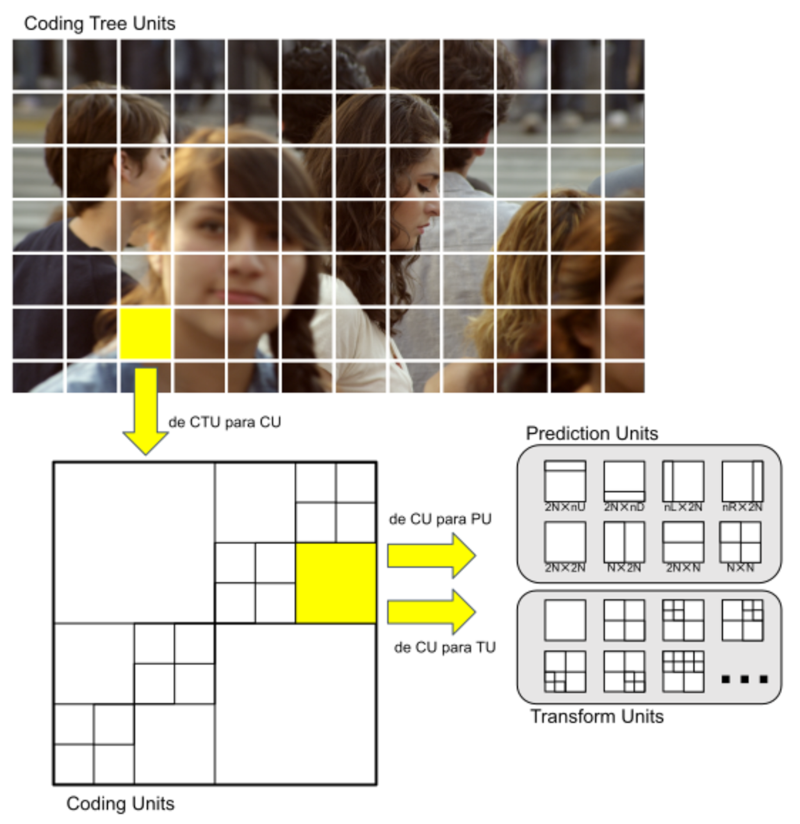
\includegraphics[width=0.85\textwidth]{FIGURES/fig_18.png}
    \caption{Exemplo de particionamento de uma CTU do H.265/HEVC. Fonte: Elaborada pelo autor.}
    \label{fig:18}
\end{figure}

No entanto, dentre todas essas estruturas de particionamento disponíveis no H.265/HEVC, é a CU que mais interessa a solução aqui apresentada, pois é essa estrutura que possibilita a identificação das regiões de agrupamento de pixels e, consequentemente, semelhante a profundidade de uma árvore de particionamento. Dessa forma, foi realizada uma avaliação de correlação entre os tamanhos de blocos observados na CU do H.265/HEVC, convertidos em profundidades com valores iguais ao do AV1, e das profundidades da árvore de particionamento do AV1. Essa avaliação está resumida na Figura \ref{fig:19}, na qual quanto mais intenso a cor, maior é a correlação entre as profundidades observadas. Logo, observa-se que quando o H.265/HEVC opta por algum tamanho de CU, os tamanhos de blocos observados no codificador AV1 tendem a serem iguais (diagonal destacada). Por exemplo, ao notar-se, durante a decodificação, a utilização da CU de tamanho 32$\times$32 (convertido para profundidade 2), em 58,09\% das vezes o codificador AV1, durante a transcodificação, também irá optar por algum arranjo de particionamentos na profundidade 2. Mas existe algumas vezes (19,21\%) em que o AV1 decide expandir a árvore de particionamentos para uma profundidade maior (de nível 3). Em raras exceções, quando o H.265/HEVC utiliza uma CU de 32$\times$32 (profundidade 2), o AV1 decide utilizar blocos de 4$\times$4 (profundidade 5), mais explicitamente, em 0,18\% das vezes. Desta forma, cada linha da Figura \ref{fig:19} representa todas as probabilidades de escolha por parte do AV1, para cada profundidade observada no decodificador H.265/HEVC.

\begin{figure}
    \centering
    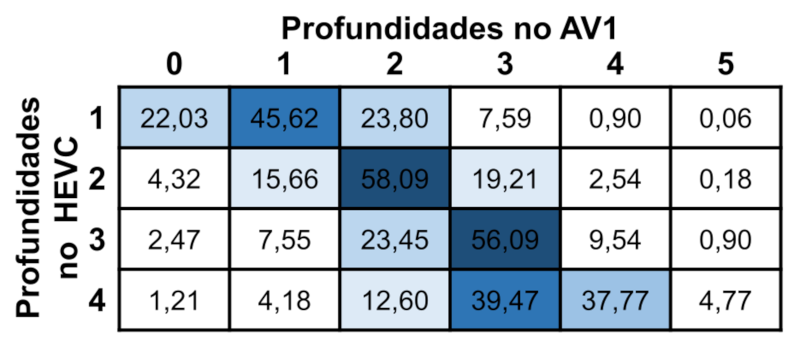
\includegraphics[width=0.75\textwidth]{FIGURES/fig_19.png}
    \caption{Correlação entre a profundidade observada na decodificação H.265/HEVC (sob QP 22) e na recodificação do mesmo vídeo para o formato AV1 (sob CQ 20). Fonte: Elaborada pelo autor.}
    \label{fig:19}
\end{figure}

Identificando-se uma correlação entre as profundidades observadas durante a decodificação e a profundidade escolhida no codificador, durante uma transcodificação, hipotetizamos que é possível inferir nas melhores profundidades a serem melhor exploradas preditivamente pelo codificador do AV1. No entanto, como vimos na Figura \ref{fig:19} e ressaltado no parágrafo anterior, todas as profundidades podem ser escolhidas pelo AV1, independentemente da profundidade observada no decodificador H.265/HEVC. Logo, propõe-se um transcodificador que considere profundidades a mais ou a menos ao observado durante a decodificação, a fim de obter transcodificadores rápidos de acordo com as necessidades de quem transcodifica os vídeos.

\subsection{Metodologia}
\label{cap:6.1.1}

Considerando o tamanho de CU observado no decodificador H.265/HEVC, cujo valor é convertido para profundidades de 1 (CU igual a 64$\times$64) até 4 (CU igual a 8$\times$8), a estratégia baseia-se em inferir as profundidades permitidas para exploração na codificação AV1. Essa profundidade observada denominaremos de $DLmap$. Como apresentamos na Figura \ref{fig:19}, na estratégia proposta o codificador AV1 pode optar por utilizar profundidades maiores que o observado em $DLmap$ ou por profundidades menores que o observado em $DLmap$. Em outras palavras, o codificador AV1 poderá optar por qualquer nível de profundidade que esteja algum nível acima ao observado em $DLmap$ (denominada como $La$, do inglês \textit{Levels Above}) ou que esteja níveis abaixo ao observado no $DLmap$ (denominado como $Lb$, do inglês, \textit{Levels Below}). Logo, a profundidade escolhida pelo codificador AV1 (denominada como $DLn$) será algum valor entre $DLmap - La$ e $DLmap + Lb$, para quaisquer valores de $La$ e $Lb$ que estejam entre 0 e 4.

A proposta desta solução é, portanto, averiguar o quão estreita pode ser a faixa de valores $La$ e $Lb$, de forma a permitir uma transcodificação rápida de H.265/HEVC para AV1. Os valores permitidos para as variáveis $La$ e $Lb$ são os mesmos: 0, 1, 2, 3 e 4. O valor 0 obriga que o codificador utilize a profundidade superior ($La$) ou a profundidade inferior ($Lb$) igual à observada na decodificação ($DLmap$); já o valor 4 indica que nenhum limite será imposto. Há, dessa forma, várias combinações de valores de $La$ e $Lb$ – mais precisamente, 25 combinações. Para identificar cada uma dessas combinações, utilizaremos a definição $La$:$Lb$, conforme a Equação \ref{eq:8}:

\begin{equation}
    \label{eq:8}
    La:Lb = \{ DLmap - La \leq DLn \leq DLmap + Lb | La, Lb \in \{ 0, 1, 2, 3, 4 \} \}
\end{equation}

Para exemplificar, consideremos um $La$:$Lb$ igual a 2:3. Então, ao observar no decodificador o uso da CU de tamanho 16$\times$16 ($DLmap$ = 3), isso significa que o codificador, naquela área do vídeo, poderá considerar realizar as predições intraquadro ou interquadros para qualquer tamanho de bloco que esteja dentro da profundidade 1 ($DLmap - La$ = 3 - 2) até a profundidade 6 ($DLmap + Lb$ = 3 + 3). Contudo, como não existe profundidade 6 no AV1, o codificador não sofrerá intervenções para exploração de profundidades além do $DLmap$. É possível observar que algo similar pode acontecer com o limite $DLmap - La$: caso La seja maior que $DLmap$, o limite retornado será negativo. Neste caso, não haverá qualquer interferência no limite superior da árvore de particionamentos

Ao assumir os limites $La$:$Lb$ estabelecidos no parágrafo anterior, é possível estimar o percentual de correlação a ser atingida por cada uma das combinações de $La$:$Lb$, com base nos valores da Figura \ref{fig:19}. Esse percentual de correlações estimadas pode ser visto na Tabela \ref{tab:IX}, onde podemos ver que a combinação 4:4, que é a mais permissiva, não se diferencia de uma transcodificação original (sem restrições). Já a transcodificação mais restritiva (combinação 0:0), tende a apresentar 49,39\% das mesmas profundidades observadas na transcodificação original. Olhando para todos os valores da Tabela \ref{tab:IX}, podemos ver que restringir o limite superior da árvore de particionamentos para $DLmap$, ou seja, $La$=0, faz com que em nenhuma combinação de $La$:$Lb$ atinja-se algum percentual de correlação acima dos 67\%. Em outras palavras, em aproximadamente um terço das profundidades que o transcodificador rápido escolher usar, haverá divergência das profundidades observadas na transcodificação original (sem restrições), caso não seja permitida alguma flexibilidade para considerar profundidades menores que aquelas observadas na decodificação.

\begin{table}
\begin{center}
\caption{Correlação (em porcentagem) estimada com diferentes combinações de $La$ e $Lb$.}
\label{tab:IX}
\footnotesize

\begin{tblr}{
 colspec = {r|r|r|r|r|r|r},
 hlines,
 row{even} = {gray9}
}
\hline
\SetCell[c=2,r=2]{} && \SetCell[c=5]{c}\textbf{Níveis Acima (La)} \\
 && 0 & 1 & 2 & 3 & 4 \\
\SetCell[r=5]{c} \textbf{Níveis Abaixo (Lb)} & 0 & 49,39 & 74,55 & 80,66 & 82,33 & 82,63 \\
 & 1 & 63,72 & 88,88 & 94,99 & 96,66 & 96,96 \\
 & 2 & 66,48 & 91,63 & 97,75 & 99,41 & 99,72 \\
 & 3 & 66,75 & 91,9 & 98,02 & 99,68 & 99,99 \\
 & 4 & 66,77 & 91,92 & 98,04 & 99,7 & 100,00 \\
\hline
\end{tblr}
\end{center}
\end{table}


Para possibilitar a aplicação dos limites La:Lb, expressos na Equação \ref{eq:8}, de forma a possibilitar ao codificador que seja encontrada a melhor profundidade ($DLn$ final) de forma rápida, propusemos o algoritmo exemplificado no fluxograma da Figura \ref{fig:20}. Nesta figura, é possível identificar três pontos de convergência:

\begin{enumerate} [1.]
    \item Caso o $DLn$ atual seja menor que o limite superior ($DLmap - La$), aplica-se o subparticionamento do bloco. No entanto, o modo simples da predição intraquadro e interquadros deve ser aplicado;
    
    \item Caso o $DLn$ atual seja maior que o limite inferior ($DLmap + Lb$), proíbe-se o subparticionamento do bloco e encerra-se o fluxo de particionamentos;

    \item Caso os limites superiores ou inferiores estejam fora dos limites de profundidade existentes, ignora-se a limitação
    
\end{enumerate}

\begin{figure}
    \centering
    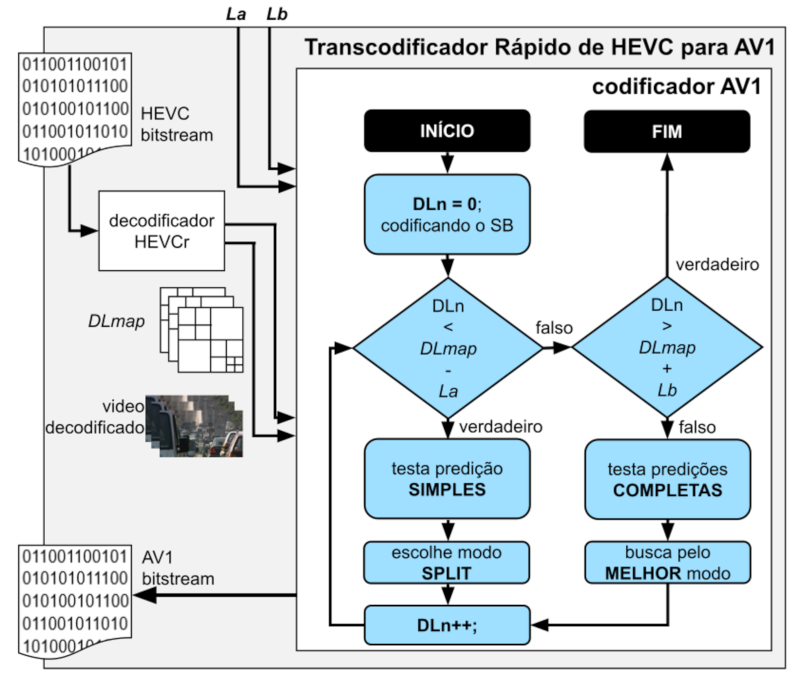
\includegraphics[width=0.75\textwidth]{FIGURES/fig_20.png}
    \caption{Fluxograma da proposta de transcodificador rápido de vídeo de H.265/HEVC para AV1 baseado em heurísticas. Fonte: Elaborada pelo autor.}
    \label{fig:20}
\end{figure}

Observe que, caso o primeiro condicional, apresentado na Figura \ref{fig:20}, seja verdadeiro, identificamos a obrigatoriedade de o codificador AV1 realizar ao menos um único modo de predição, o qual denominamos de modo simples. O modo simples da predição intraquadro é o modo \texttt{DC} e o modo simples da predição interquadros é o  modo \texttt{NEARESTMV}, estes modos foram escolhidos por serem os primeiros modos a serem testados nestas etapas de predição.  Essa predição obrigatória serve como garantia de que o valor obtido durante o cálculo do custo taxa-distorção (do inglês, \textit{rate-distortion cost}, ou rd-cost) seja corretamente gerado, principalmente após os subparticionamentos de blocos. Isso é necessário, pois é através do cálculo de rd-cost que o codificador identifica quais combinação de árvores de profundidades e seus respectivos modos preditivos são melhores para serem aplicados em um determinado momento da codificação, para um determinado conteúdo. No entanto, se aplicarmos diretamente o subparticionamento dos primeiros níveis de profundidade da árvore sem a obtenção de qualquer valor de rd-cost, o codificador não estará apto a decidir se aquela combinação de árvore e de modos preditivos é melhor ou pior que outra, podendo entrar em uma situação impossível (por exemplo, uma repetição infinita).

\subsection{Resultados}
\label{cap:6.1.2}

Para verificar a eficiência da proposta de transcodificador rápido, os primeiros 60 quadros de quatro sequências de vídeos HD1080 foram utilizados para realização do experimento, utilizando a versão 1.0.0 do software de referência do codificador AV1. Os resultados deste experimento podem ser vistos na Tabela \ref{tab:X}, onde todas as combinações de La:Lb estão ordenadas por redução do tempo de transcodificação (TS). De forma geral, é possível observar que existe uma tendência de aumento proporcional entre o TS e o BD-rate, principalmente quando há uma maior restrição entre os valores de $La$ e de $Lb$, o que é facilmente explicável, já que se reduz significativamente a quantidade de blocos disponíveis para testes. 

Como esperado, a combinação mais permissiva (4:4) não se diferencia da transcodificação sem intervenções e, por outro lado, a combinação mais restritiva (0:0) apresenta maior TS e, consequentemente, maior BD-rate. Já a combinação 2:2, intermediária entre essas duas, é discreta em seus resultados, acelerando apenas 5\% a um custo de reduzir a eficiência de codificação em 0,1145\%. O único caso que apresentou resultados fora do esperado é a combinação 3:4, cujo tempo de transcodificação rápido pode ser considerado uma variação normal de execução do software, com 0,20\% em relação à transcodificação original. Contudo, essa combinação apresentou um BD-rate negativo (de -0,0128\%), ou seja, mostrou-se mais eficiente em codificar o vídeo decodificado que a versão de codificação de referência. Analisando-se os dados brutos, identificou-se que a combinação 3:4 apresentou bons resultados em sequências de menor variação de movimento, onde os vídeos possuem mais movimento de câmera do que de objetos.

\begin{table}
\begin{center}
\caption{Resultados das transcodificações H,265/HEVC para AV1 sob diferentes combinações de $La:Lb$.}
\label{tab:X}
\footnotesize

\begin{tblr}{
    colspec = {c|r|r|r},
    hlines,
    row{even} = {gray9}
}
\hline
\textbf{$La:Lb$} & \textbf{BD-rate (\%)} & \textbf{TS (\%)} & \textbf{Razão} \\
0:0 & 14,6688 & 61,20 & 0,240 \\
2:0 & 5,0935 & 40,80 & 0,125 \\
3:0 & 5,0628 & 40,70 & 0,124 \\
4:0 & 5,0215 & 40,00 & 0,126 \\
1:0 & 6,1817 & 39,80 & 0,155 \\
0:1 & 6,1688 & 32,00 & 0,193 \\
1:1 & 1,1950 & 21,00 & 0,057 \\
0:2 & 3,9088 & 20,00 & 0,195 \\
2:1 & 0,8708 & 18,00 & 0,048 \\
3:1 & 0,8703 & 17,70 & 0,049 \\
4:1 & 0,9020 & 17,70 & 0,051 \\
0:3 & 3,5850 & 15,40 & 0,233 \\
0:4 & 3,5125 & 15,10 & 0,233 \\
1:2 & 0,4263 & 8,00 & 0,053 \\
2:2 & 0,1145 & 5,00 & 0,023 \\
3:2 & 0,0645 & 4,60 & 0,014 \\
4:2 & 0,0583 & 4,60 & 0,013 \\
1:4 & 0,3180 & 3,50 & 0,091 \\
1:3 & 0,3308 & 3,50 & 0,094 \\
2:3 & 0,0070 & 0,50 & 0,014 \\
3:3 & 0,0043 & 0,40 & 0,011 \\
2:4 & 0,0050 & 0,30 & 0,017 \\
4:3 & 0,0493 & 0,30 & 0,164 \\
3:4 & -0,0128 & 0,20 & -0,064 \\
4:4 & 0,0000 & 0,00 & \SetCell[c=1]{c}-~- \\
\hline
\end{tblr}
\end{center}
\end{table}


A relação existente entre o TS atingido e o impacto no BD-rate, na Tabela \ref{tab:X}, pode ser observado através da coluna Razão. Conforme já foi apresentado no capítulo \ref{cap:3}, Razão indica o acréscimo de BD-rate para cada percentual de tempo acelerado. Portanto, quanto menor esse valor, melhor tende a ser a solução proposta para transcodificação rápida. Observando apenas o valor de Razão, a melhor combinação (exceto a 3:4) é a 3:3, que impacta em 0,011\% de BD-rate para cada percentual de tempo reduzido. Todavia, essa combinação tem potencial de aceleração inferior a 0,5\% do tempo de transcodificação original, ou seja, também pode ser considerada uma variação normal da execução do software. Considerando os resultados de TS superiores a 5\%, a combinação 2:2 é a melhor, com um aumento de 0,023\% de BD-rate para cada percentual de tempo reduzido. Nota-se, inclusive, que todas as combinações com $Lb$ igual ou superior a 2 atingem menos de 10\% de aceleração. Ou seja, autorizar que o \textit{libaom} considere blocos de um nível de profundidade muito além do observado na decodificação não traz ganhos significativos de tempo. Por outro lado, permitir apenas uma única profundidade além do observado ($Lb$=1) possibilita atingir TS moderados (entre 10\% e 20\%). Já ganhos significativos de TS (30\% ou mais) se apresentam somente quando não se permite testar nenhuma profundidade além daquela observada ($Lb$=0). Essas três observações pontuais são relevantes para a definição da metodologia de transcodificação rápida com uso de aprendizado de máquina (capítulo \ref{cap:7}).

O único trabalho disponível para comparação com a nossa proposta de transcodificador rápido de H.265/HEVC para AV1 foi desenvolvido por \citet{bib:chen_2019}, que propôs duas abordagens em seu trabalho. Na primeira abordagem, o autor limita as profundidades máximas e mínimas da árvore de particionamento do codificador AV1 com base no histórico de profundidades observadas na decodificação HEVC. Basicamente, o autor aplica, quadro a quadro, uma análise probabilística de ocorrência de cada uma das profundidades observadas anteriormente, considerando pesos menores a quadros mais distantes ao quadro atual em codificação. Assim, obtém uma estimativa de quais profundidades não precisam ser consideradas na avaliação do codificador AV1. Ainda nessa primeira abordagem, caso a profundidade seja superior ao limite estimado no trabalho, o autor desabilita os testes de predição interquadros com particionamentos não-quadráticos. Já na segunda abordagem, \citet{bib:chen_2019} utiliza um modelo de inferência bayesiana condicional \cite{bib:bayesian_ref} para identificar o fim do particionamento de blocos. Segundo \citet{bib:chen_2019}, essa segunda abordagem foi inspirada no trabalho de \cite{bib:guo2_2018}, que utilizou um modelo de inferência bayesiana condicional para reduzir a complexidade do processo de particionamento do codificador AV1, ainda em suas versões iniciais (pré v1.0.0). Dessa forma, \citet{bib:chen_2019} obtém uma aceleração de 37,8\% da transcodificação a um custo de elevar o BD-rate em apenas 0,79\%, conforme já apresentamos na seção \ref{cap:3.1}. Logo, apesar da primeira abordagem do autor ser similar à nossa, a forma como se dá a análise estatística é diferente. Enquanto \citet{bib:chen_2019} realiza uma análise estatística local, quadro a quadro e em tempo de execução, a nossa proposta considera uma análise estatística de vídeos inteiros e diferentes ao que se está codificando no momento. Ainda assim, os resultados apresentados por \citet{bib:chen_2019} se assemelham à nossa combinação 2:2 (0,1145\% de BD-rate e 5,00\% de TS) ou à combinação 2:4 (0,0050 de BD-rate e 0,30\% de TS), pois \citet{bib:chen_2019} apresenta uma Razão de 0,0020\% de BD-rate para cada porcento de redução de tempo. Todavia, apesar de proporcionalmente \citet{bib:chen_2019} apresentar valores similares aos nossos, o autor obtém um TS superior.

\subsection{Ajuste de Complexidade Experimental}
\label{cap:6.1.3}

Por fim, considerando os resultados apresentados no transcodificador de H.265/HEVC para AV1, baseado em permissões de profundidade máxima ($La$) e mínima ($Lb$) da árvore de particionamentos, demonstrados na subseção anterior, avaliamos também um cenário de ajuste de complexidade em tempo de codificação. A ideia principal consiste em  disponibilizar as diversas combinações de $La$:$Lb$ para prover uma transcodificação rápida de acordo com as necessidades do usuário. Para tanto, realizamos um experimento utilizando as combinações 2:0, 1:1 e 1:2 durante a codificação da sequência de vídeo \textit{Tennis} (de resolução HD1080). A escolha dessas combinações se deu por serem as primeiras combinações $La$:$Lb$ a apresentarem resultados de TS próximos de 40\%, 20\% e 10\%. Foi realizada uma troca de combinação a cada 20 quadros de vídeo codificado e, dessa forma, foi possível acelerar 22,75\% do tempo de transcodificação a um custo de elevar o BD-rate em 5,49\%. Na Figura \ref{fig:22}, mostramos a variação do tempo de codificação de cada quadro do vídeo ao longo de toda a transcodificação; a linha azul representa a transcodificação original e a linha laranja a transcodificação rápida. Desta forma, é possível observar, na Figura \ref{fig:22}, que o trecho transcodificado com a combinação 2:0 (fundo em verde) apresenta a maior diferença de tempo de codificação, ou seja, a linha laranja está nítidamente abaixo da linha azul. No entanto, conforme utilizam-se combinações menos restritivas, a diferença no tempo de codificação também reduz, ficando quase idêntico ao tempo observado na transcodificação de referência, como era esperado que ocorresse. Desta forma, torna-se evidente que a utilização desta técnica para acelerar um transcodificador utilizando combinações $La$:$Lb$, ajustando os valores dessas combinações conforme a necessidade do operador em diferentes momentos do vídeo, é possível e eficiente em termos de redução de complexidade. Todavia, o BD-rate gerado não é diretamente calculável, assumindo-se um teto médio da combinação, conforme apresentado na Tabela \ref{tab:X}.

\begin{figure}
    \centering
    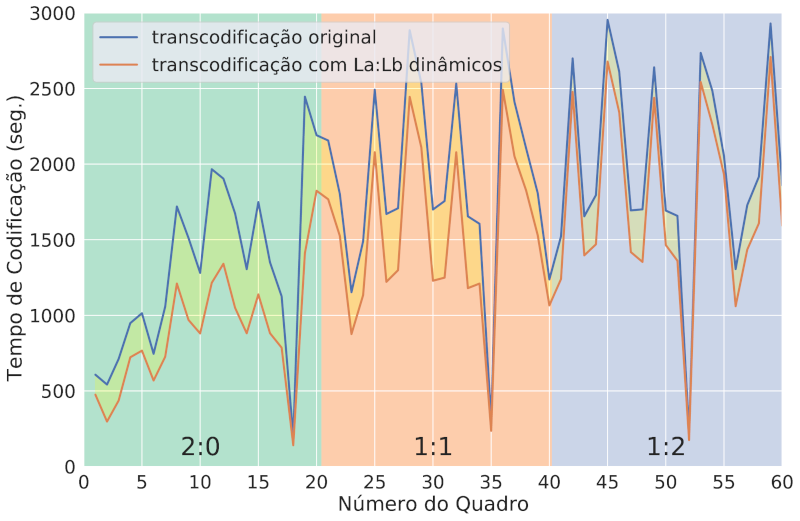
\includegraphics[width=0.75\textwidth]{FIGURES/fig_22.png}
    \caption{Relação do tempo de transcodificação quadro a quadro, comparando a transcodificação original com a transcodificação com troca dinâmica de $La:Lb$. Fonte: Elaborada pelo autor.}
    \label{fig:22}
\end{figure}
